% Template for Latex
% Document author - Nagendra Krishnamurthy

\documentclass[12pt]{article}

\setlength{\textwidth}{6.5in}
\setlength{\textheight}{8.75in}
\setlength{\evensidemargin}{0in}
\setlength{\oddsidemargin}{0in}
\setlength{\topmargin}{0in}

\setlength{\parindent}{0pt}
\setlength{\parskip}{0.1in}

\title{NSEG-5984 Monte Carlo Methods for Particle Transport}
%\subtitle{Homework 1}
\author{Nagendra Krishnamurthy}

% Uncomment for double-spaced document.
% \renewcommand{\baselinestretch}{2}

\usepackage[latin1]{inputenc}
\usepackage{tikz}
\usetikzlibrary{shapes,arrows}
\usepackage{epstopdf}
% \usepackage{epsf}
% \usepackage{glossaries}
\usepackage{graphicx}
\usepackage{scalefnt}

\definecolor{Brown}{cmyk}{0,0.81,1,0.60}
\definecolor{OliveGreen}{cmyk}{0.64,0,0.95,0.40}
\definecolor{CadetBlue}{cmyk}{0.62,0.57,0.23,0}
\definecolor{lightlightgray}{gray}{0.9}

\usepackage{listings}
\lstset{frame=shadowbox, rulesepcolor=\color{blue}}
\lstset{ %
language=[90]Fortran,           % the language of the code
basicstyle=\scriptsize\ttfamily,           % the size of the fonts that are used for the code
%numbers=left,                  % where to put the line-numbers
numberstyle=\scriptsize,      % the size of the fonts that are used for the line-numbers
stepnumber=2,                   % the step between two line-numbers. If it's 1, each line 
                                % will be numbered
numbersep=5pt,                  % how far the line-numbers are from the code
backgroundcolor=\color{lightlightgray},  % choose the background color. You must add \usepackage{color}
showspaces=false,               % show spaces adding particular underscores
showstringspaces=false,         % underline spaces within strings
showtabs=false,                 % show tabs within strings adding particular underscores
frame=single,                   % adds a frame around the code
tabsize=2,                      % sets default tabsize to 2 spaces
captionpos=b,                   % sets the caption-position to bottom
breaklines=true,                % sets automatic line breaking
breakatwhitespace=false,        % sets if automatic breaks should only happen at whitespace
title=\lstname,                 % show the filename of files included with \lstinputlisting;
                                % also try caption instead of title
escapeinside={\%*}{*)},         % if you want to add a comment within your code
keywordstyle=\color{OliveGreen}, % Keywords font ('*' = uppercase)
morekeywords={*,...}           % if you want to add more keywords to the set
}
% \usepackage{natbib}

% \makeglossaries

% \newglossaryentry{cd}{name=$C_D$,description={Coefficient of drag}}
% \newglossaryentry{cl}{name=$C_L$,description={Coefficient of lift}}

\begin{document}

\maketitle

\textbf{Problem 1:}
\textit{Diagram a flowchart for an algorithm for randomly selecting
the sums of the top faces (n1,n2) on a pair of well-balanced cubical
dice based on generated random numbers h's. Write a program to obtain
the pdf for the random variable s (=n1+n2).}

% Define block styles
\tikzstyle{decision} = [diamond, draw, fill=blue!20, aspect=2,
    text width=4.5em, text badly centered, node distance=1.5cm, inner sep=0pt]
\tikzstyle{block} = [rectangle, draw, fill=blue!20, 
    text width=12em, text centered, rounded corners, minimum height=2em]
\tikzstyle{line} = [draw, -latex']
\tikzstyle{cloud} = [draw, ellipse,fill=red!20, node distance=3cm,
    minimum height=2em]

\begin{center}
{\scalefont{0.75}
\begin{tikzpicture}[node distance = 1.5cm, auto]
    % Place nodes
    \node [block] (start) {Start};
    \node [block, below of=start] (init) {iter = 0};
    \node [block, below of=init] (generate) {Generate $\eta_1$ and
    $\eta_2$};
    \node [block, below of=generate] (compute) {
    $n_1 = $ INT$(6 \times \eta_1 ) + 1$ \\
    $n_2 = $ INT$(6 \times \eta_2 ) + 1$};
    \node [block, below of=compute] (sum) {s = $n_1$ + $n_2$};
    \node [block, below of=sum] (print) {count(s) = count(s) + 1};
    \node [block, below of=print] (iterIncrement) {iter = iter + 1};
    \node [decision, below of=iterIncrement] (iterCheck) {Is iter $<$
    iterMax?};
    \node [block, below of=iterCheck] (pdfCompute) {pdf(:) =
    count(:)/iterMax};
    \node [block, below of=pdfCompute] (stop) {Stop};

    % Draw edges
    \path [line] (start) -- (init);
    \path [line] (init) -- (generate);
    \path [line] (generate) -- (compute);
    \path [line] (compute) -- (sum);
    \path [line] (sum) -- (print);
    \path [line] (print) -- (iterIncrement);
    \path [line] (iterIncrement) -- (iterCheck);
    \path [line] (iterCheck) -- node {no} (pdfCompute);
    \path [line] (iterCheck.west) -- +(-3,0) node [near start] {yes} |- (generate.west);
    \path [line] (pdfCompute) -- (stop);
\end{tikzpicture}
}
\end{center}

Source code:
\lstinputlisting{problem_1.f90}

The following plot provides the probability density function obtained.
The code was executed for iterMax = 1000000.

\begin{center}
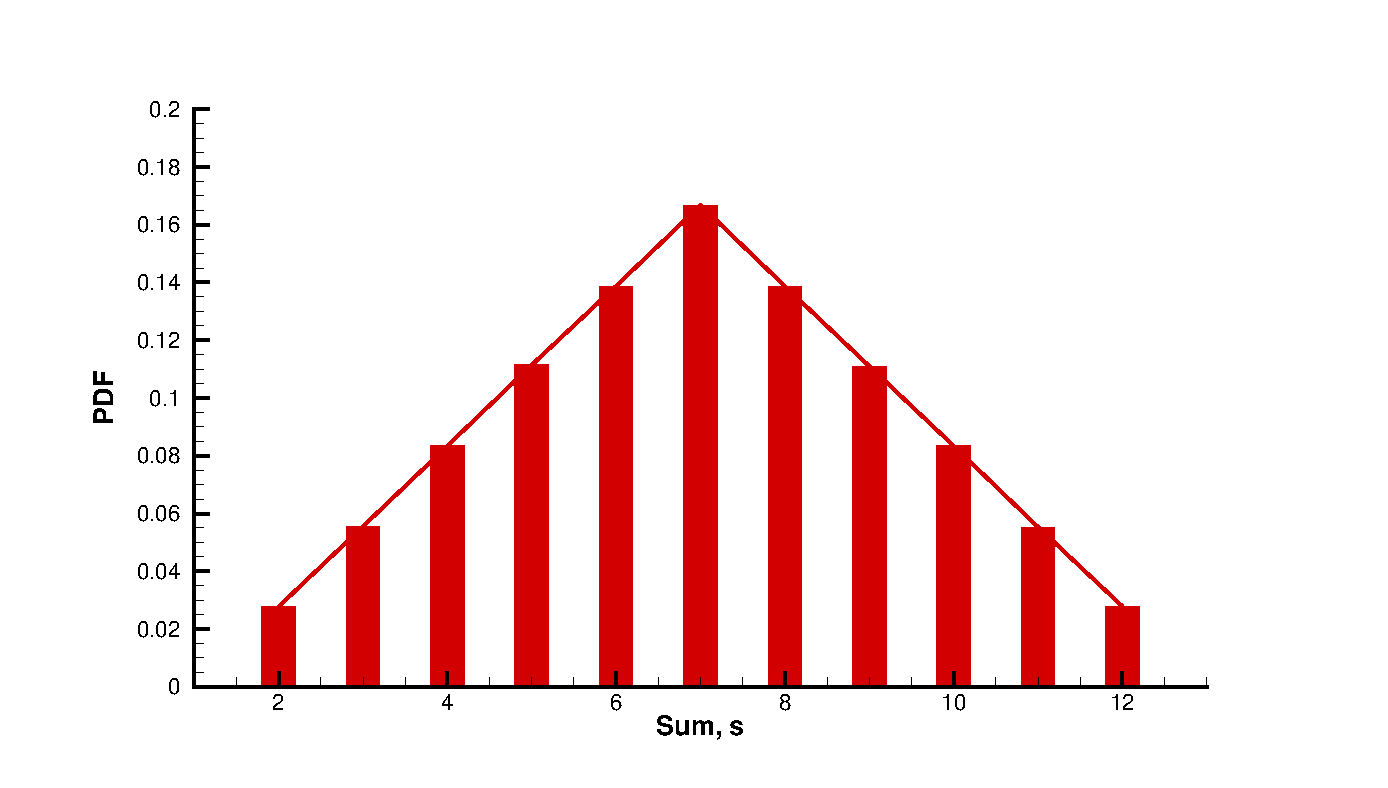
\includegraphics[width=0.7\textwidth]{plot1_bar.eps}
\end{center}

\textbf{Problem 2:}
\textit{Diagram a flowchart and write a program for an algorithm
for randomly selecting a "flush poker" hand based on generated random
numbers, $\eta$'s, considering that all cards are from the same suit. A
flush poker hand consists of 5 cards from a deck of 52 cards. A deck
consists of 13 cards in each of 4 suits, spades, hearts, diamonds, and
clubs. The 13 cards in each suit are numbered from 1 to 10 plus jack,
queen, and king.}

% Define block styles
\tikzstyle{decision} = [diamond, draw, fill=blue!20, aspect=2,
    text width=8.5em, text centered, node distance=1.5cm, inner sep=0pt]
\tikzstyle{block} = [rectangle, draw, fill=blue!20, 
    text width=16em, text centered, rounded corners, minimum height=1em]
\tikzstyle{line} = [draw, -latex']
\tikzstyle{cloud} = [draw, ellipse,fill=red!20, node distance=3cm,
    minimum height=2em]

\begin{center}
{\scalefont{0.75}
\begin{tikzpicture}[node distance = 1.5cm, auto]
    % Place nodes
    \node [block] (start) {Start\\
    iter = 0};
    \node [block, below of=start] (initialize) {
    Create list of cards\\
    i = 0; iter = iter + 1};
    \node [block, below of=initialize] (iIncrement) {$i=i+1$};
    \node [block, below of=iIncrement] (genRand) {Generate random
    number $\eta_i$};
    \node [block, below of=genRand] (findCard) {Find card number \\
    $c_i=$ INT$(52-i+1)+1$};
    \node [block, below of=findCard] (addDelCard) {Append card to list
    of chosen cards\\
    Delete card from full list};
    \node [decision, below of=addDelCard, node distance=2.0cm] (checkCard) {Are all chosen
    cards of same suit?};
    \node [decision, below of=checkCard, node distance = 2.0cm] (checkNumCards) {$i<5?$};
    \node [block, below of=checkNumCards, node distance = 2 cm]
    (success) {success = success + 1};
    \node [decision, below of=success, node distance = 2 cm]
    (countCheck) {Is iter $<$ iterMax?};
    \node [block, below of=countCheck, node distance = 2 cm] (print) {Print probability};
    \node [block, below of=print] (stop) {Stop};

    % Draw edges
    \path [line] (start) -- (initialize);
    \path [line] (initialize) -- (iIncrement);
    \path [line] (iIncrement) -- (genRand);
    \path [line] (genRand) -- (findCard);
    \path [line] (findCard) -- (addDelCard);
    \path [line] (addDelCard) -- (checkCard);
    \path [line] (checkCard) -- node {yes} (checkNumCards);
    \path [line] (checkCard.west) -- +(-2,0) node [near start] {no} |- (initialize.west);
    \path [line] (checkNumCards) -- node {yes} (success);
    \path [line] (checkNumCards.west) -- +(-2,0) node [near start]
    {no} |- (iIncrement.west);
    \path [line] (success) -- (countCheck);
    \path [line] (countCheck) -- node {no} (print);
    \path [line] (countCheck.west) -- +(-3,0) node [near start] {yes} |- (initialize.west);
    \path [line] (print) -- (stop);
\end{tikzpicture}
}
\end{center}

Source code:
\lstinputlisting{problem_2.f90}

The code was executed was various values of iterMax. From the plot, it
is concluded that the probability of a flush hand is approximately
$1.9\times10^{-3}$.

\begin{center}
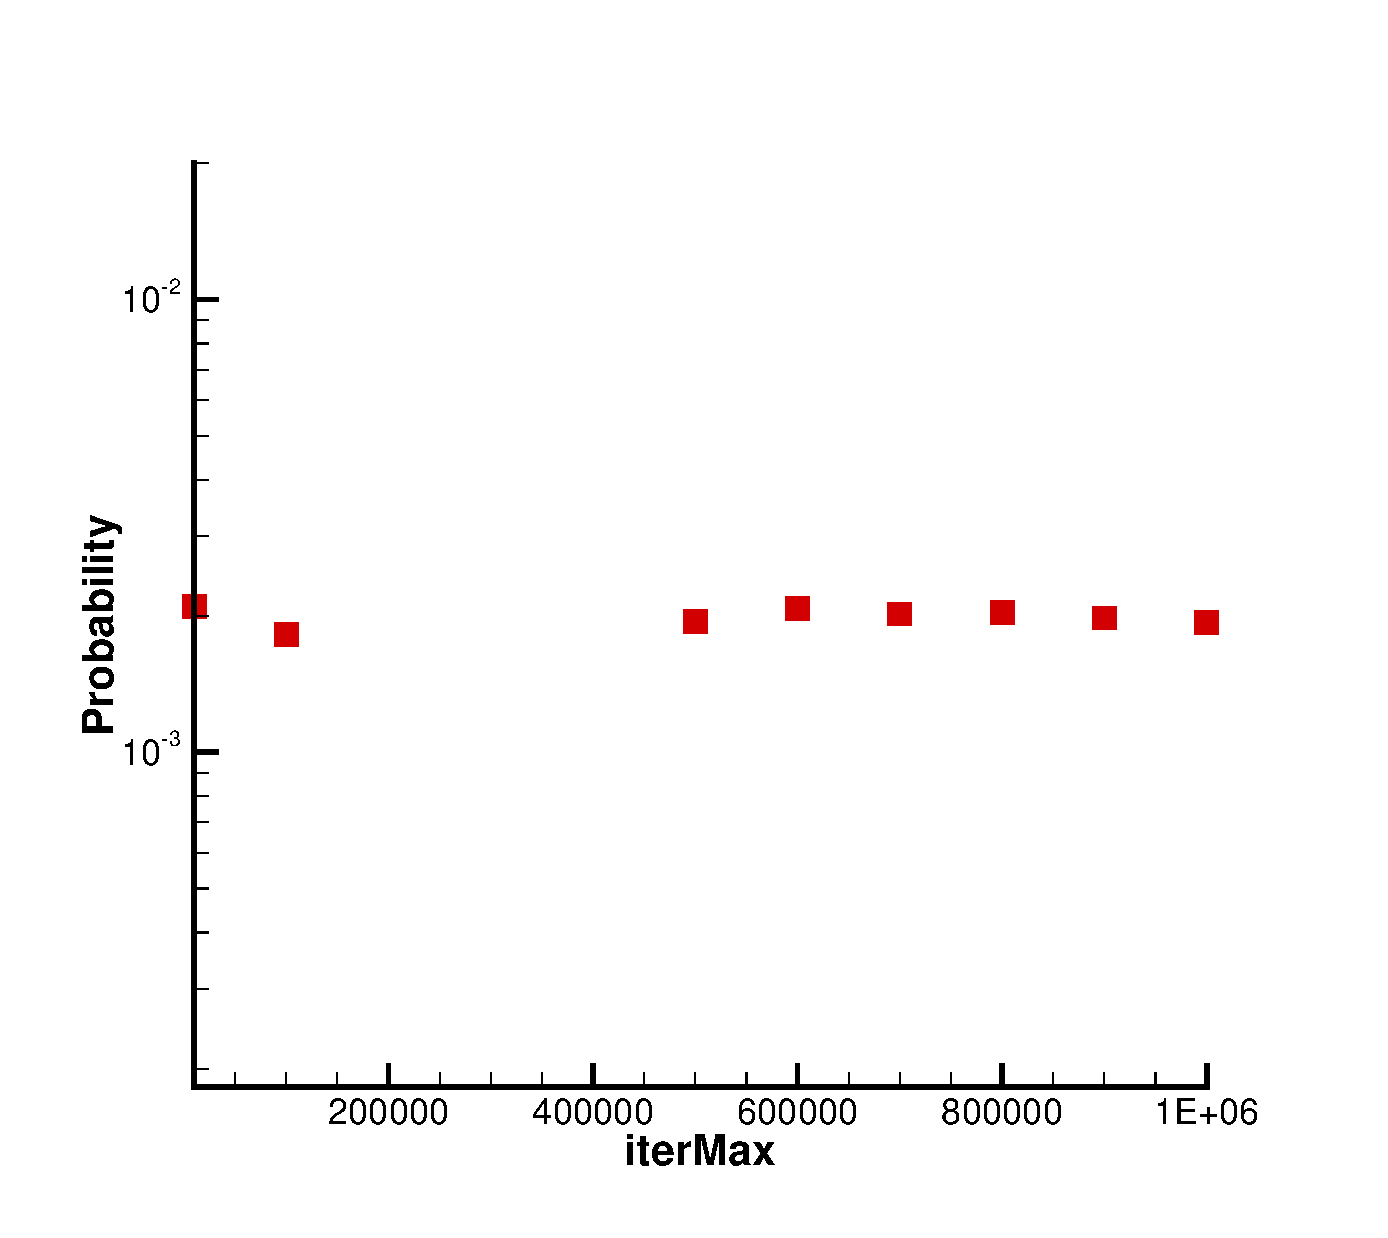
\includegraphics[width=0.7\textwidth]{probFlush.eps}
\end{center}


\textbf{Problem 3:}
\textit{Consider a continuous random variable $x$ defined in a range
$[0, 3]$ with a distribution $f(x) = x^2$.  a) Determine the pdf of this
random variable; b) Write a program for selecting $x$ using a random
number ($\eta$).}

Given distribution function:
\begin{equation}
  f(x) = x^2
  \label{eq_dist_func}
\end{equation}

Probability density function (PDF) will be given by:
\begin{equation}
  p(x) = \frac{f(x)}{\int_{0}^{3}f(x)\,dx}
\end{equation}
\begin{equation}
  p(x) = \frac{x^2}{\int_{0}^{3}x^2\,dx} =
  \frac{x^2}{\frac{x^3}{3}\bigg|_{0}^{3}}
\end{equation}
\begin{equation}
  p(x) = \frac{x^2}{9}
\end{equation}

Fundamental formulation of Monte Carlo:
\begin{equation}
  \int_{0}^{x}p(x')\,dx' = \eta
\end{equation}
\begin{equation}
  \int_{0}^{x}\frac{x'^2}{9}\,dx' = \eta
\end{equation}
\begin{equation}
  \frac{x^3}{27} = \eta
\end{equation}
\begin{equation}
  x = 3\sqrt[3]\eta
\end{equation}

Source code:
\lstinputlisting{problem_3.f90}

\begin{center}
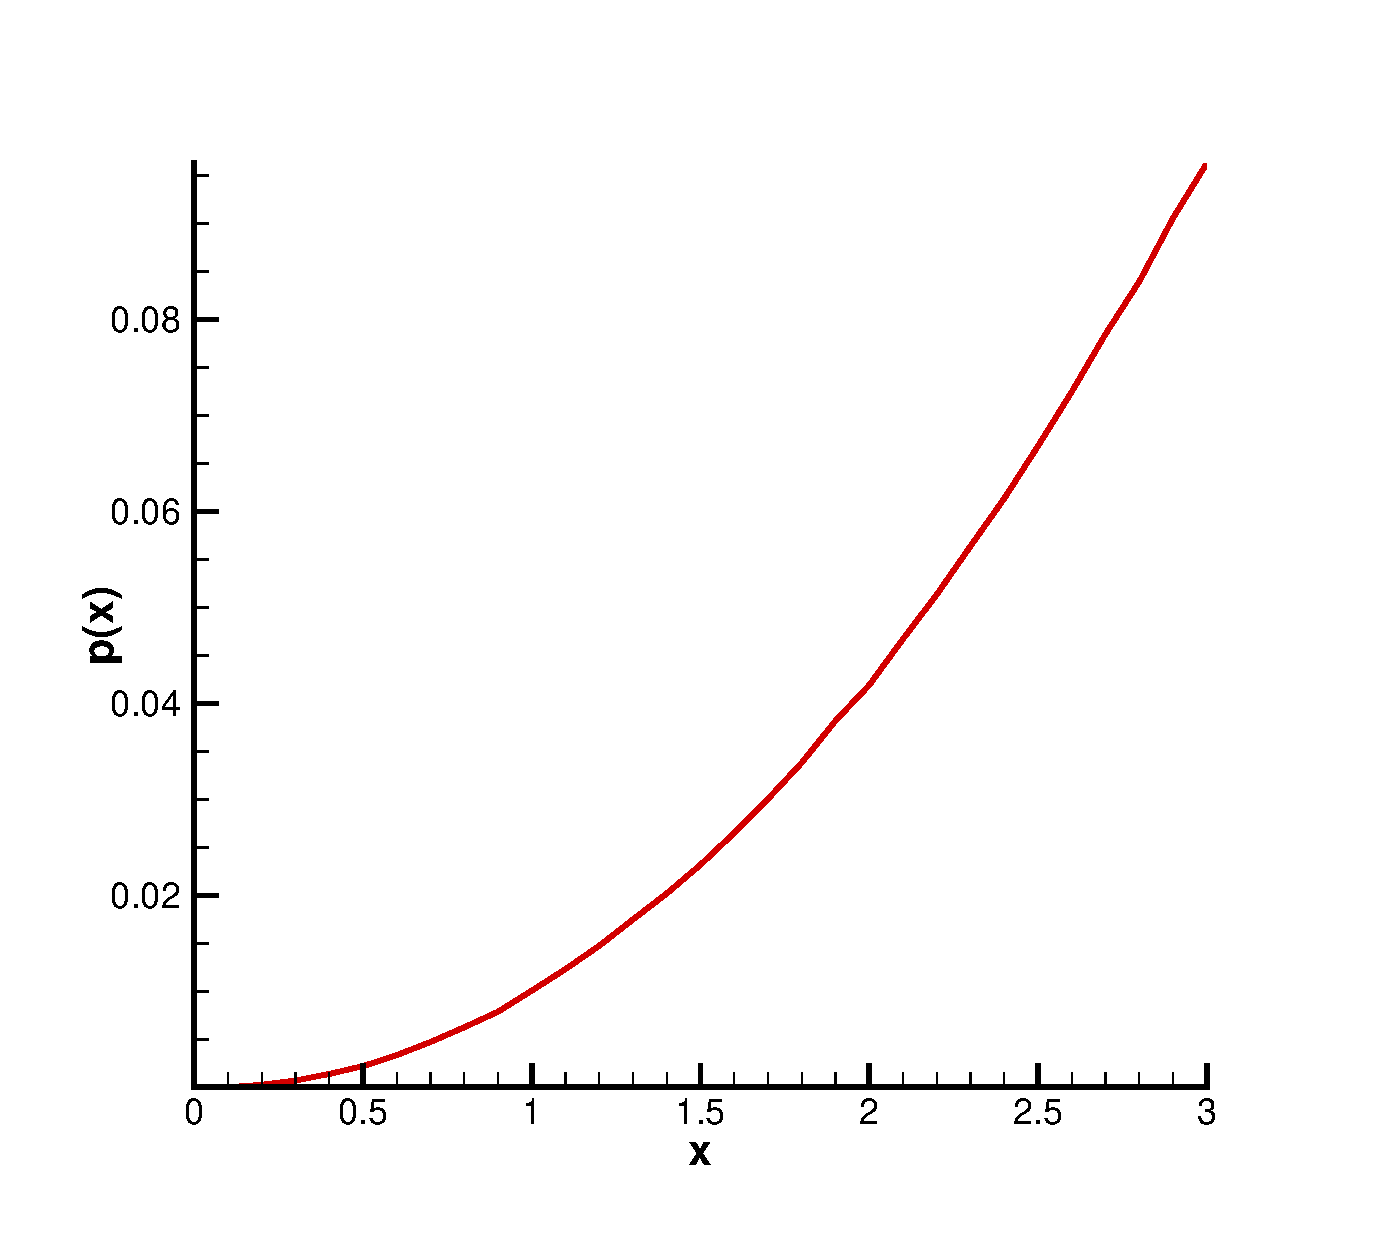
\includegraphics[width=0.7\textwidth]{pdf_x2.eps}
\end{center}


% \bibliographystyle{plainnat}
% \bibliography{path_to_bibliography}
% \printglossaries

\end{document}

